\documentclass[../main]{subfiles}
\begin{document}

\section{Qualità di processo}
Per parlare della qualità di processo si può cominciare con una semplice frase: "\textit{Da tubi sporchi non esce acqua pulita}". Nel caso dell'\g{ingegneria del software}, i tubi sono i \g{processi} mentre l'acqua è il \g{prodotto software}.\newline
Da questo concetto nasce l'esigenza di evitare che i \g{processi} siano "sporchi", ovvero non di qualità. La qualità di processo, e la sua verifica, devono far parte del ciclo di miglioramento continuo.
\begin{figure}[h]
    \begin{center}
        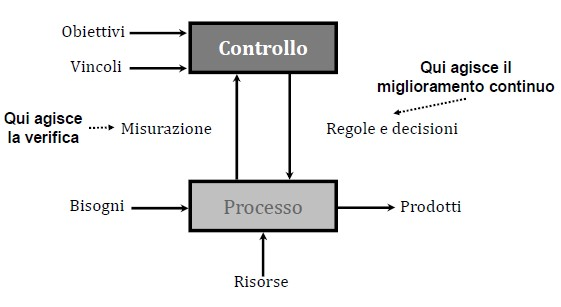
\includegraphics[scale=0.8]{immagini/processo.jpg}
    \end{center}
\end{figure}
Il miglioramento continuo è necessario per migliorare costantemente i \g{processi} e il \g{way of working}, anche se comunque è bene che quest'ultimo sia già buono in partenza (ispirato da standard e \g{best practice}) per i processi primari. La \g{verifica} deve essere continua e quantitativa.\newline

\end{document}